\pdfoutput=1
% \documentclass[red,handout,professionalfont]{beamer}
\documentclass[red,professionalfont]{beamer}
\usepackage{multimedia}
\usepackage{chessboard}
\usepackage{url}
\usepackage{amssymb}  % the check symbol 
% Python listing setup

\usepackage{color}
\usepackage[procnames]{listings}
\usepackage{textcomp}
\usepackage{setspace}
\usepackage{palatino}
\renewcommand{\lstlistlistingname}{Code Listings}
\renewcommand{\lstlistingname}{Code Listing}
\definecolor{gray}{gray}{0.5}
\definecolor{green}{rgb}{0,0.5,0}
\definecolor{lightgreen}{rgb}{0,0.7,0}
\definecolor{purple}{rgb}{0.5,0,0.5}
\definecolor{darkred}{rgb}{0.5,0,0}
\lstnewenvironment{python}[1][]{
\lstset{
language=python,
breaklines=true,
basicstyle=\ttfamily\small\setstretch{1},
stringstyle=\color{green},
showstringspaces=false,
alsoletter={1234567890},
otherkeywords={\ , \}, \{},
keywordstyle=\color{blue},
emph={access,and,as,break,class,continue,def,del,elif,else,%
except,exec,finally,for,from,global,if,import,in,is,%
lambda,not,or,pass,print,raise,return,try,while,assert},
emphstyle=\color{orange}\bfseries,
emph={[2]self},
emphstyle=[2]\color{gray},
emph={[4]ArithmeticError,AssertionError,AttributeError,BaseException,%
DeprecationWarning,EOFError,Ellipsis,EnvironmentError,Exception,%
False,FloatingPointError,FutureWarning,GeneratorExit,IOError,%
ImportError,ImportWarning,IndentationError,IndexError,KeyError,%
KeyboardInterrupt,LookupError,MemoryError,NameError,None,%
NotImplemented,NotImplementedError,OSError,OverflowError,%
PendingDeprecationWarning,ReferenceError,RuntimeError,RuntimeWarning,%
StandardError,StopIteration,SyntaxError,SyntaxWarning,SystemError,%
SystemExit,TabError,True,TypeError,UnboundLocalError,UnicodeDecodeError,%
UnicodeEncodeError,UnicodeError,UnicodeTranslateError,UnicodeWarning,%
UserWarning,ValueError,Warning,ZeroDivisionError,abs,all,any,apply,%
basestring,bool,buffer,callable,chr,classmethod,cmp,coerce,compile,%
complex,copyright,credits,delattr,dict,dir,divmod,enumerate,eval,%
execfile,exit,file,filter,float,frozenset,getattr,globals,hasattr,%
hash,help,hex,id,input,int,intern,isinstance,issubclass,iter,len,%
license,list,locals,long,map,max,min,object,oct,open,ord,pow,property,%
quit,range,raw_input,reduce,reload,repr,reversed,round,set,setattr,%
slice,sorted,staticmethod,str,sum,super,tuple,type,unichr,unicode,%
vars,xrange,zip},
emphstyle=[4]\color{purple}\bfseries,
upquote=true,
morecomment=[s][\color{lightgreen}]{"""}{"""},
commentstyle=\color{red}\slshape,
literate={>>>}{\textbf{\textcolor{darkred}{>{>}>}}}3%
         {...}{{\textcolor{gray}{...}}}3,
procnamekeys={def,class},
procnamestyle=\color{blue}\textbf,
framexleftmargin=1mm, framextopmargin=1mm,% frame=shadowbox,
%rulesepcolor=\color{blue},
#1
}}{}


\usepackage{tikz}
\usepackage{tikz-qtree}
\usetikzlibrary{decorations.pathreplacing,positioning}
%\bibliography{mujstyl}
\theoremstyle{definition}
\newtheorem{definice}{Definition}[section]
\newtheorem{thm}{Theorem}[section]
\newtheorem{idea}{Idea}[section]
\newtheorem{cor}[thm]{Corrollary}
\newtheorem{lem}[thm]{Lemma}
\newtheorem{obs}[thm]{Observation}
\newtheorem{rem}[thm]{Remark}
\newtheorem{ex}[thm]{Example}
\newtheorem{quizz}[thm]{Question}
\newcommand{\pomega}{\mbox{$\mathcal{P}(\omega)$}}
\newcommand{\cont}{\mbox{$\mathfrak c$}}
\newcommand{\ba}{\mbox{${\mathbb B}$}}
\newcommand{\0}{\mbox{${\bf 0}$}}
\newcommand{\F}{\mbox{${\mathcal F}$}}
\newcommand{\rest}{\mbox{$\upharpoonright$}}
\newcommand{\cl}[1]{\mbox{$\overline{#1}$}}
\newcommand{\yes}{\textcolor{green}{$\checkmark$}}
\newcommand{\no}{\textcolor{red}{$\times$}}
\renewcommand{\emph}[1]{{\bf #1}}
\mode<presentation>
{
\useinnertheme{rounded}

\usecolortheme{whale}
\usecolortheme{orchid}

\setbeamerfont{block title}{size={}}

%   \useoutertheme{default}
%   \usetheme{Copenhagen}
%   \useoutertheme{default}
  \setbeamercovered{invisible}
}
\setbeamertemplate{navigation symbols}{} 
\usepackage[utf8]{inputenc}
\usepackage[czech,english]{babel}
\usepackage{lmodern}
%\usepackage{times}
\usepackage[T1]{fontenc}


\tikzset{onslide/.code args={<#1>#2}{%
  \only<#1>{\pgfkeysalso{#2}} % \pgfkeysalso doesn't change the path
}}

\tikzstyle{hilight}=[red,ultra thick]
\tikzstyle{active}=[yellow,ultra thick]
\tikzstyle{memory}=[blue]



\title[]{Lokální prohledávání \\ (5. přednáška)}

% Dnes se podíváme na jednoduché "goal-based" agenty
% a ukážeme si obecné postupy 


% \author[]{Jonathan L. Verner}
% \institute[Charles University, Prague] % (optional,but mostly needed)
% {
%   Department of Logic\\
%   Faculty of Philosophy\\
%   Charles University in Prague
% }
\date[]{}
% \subject{}
%\pgfdeclareimage[height=1cm]{university-logo}{UK-logo}
%\logo{\pgfuseimage{university-logo}}

\begin{document}

\AtBeginSection[]
{
  \begin{frame}<beamer>
    \begin{block}{}
%    \begin{centering}
    \hfill\insertsection\hfill\
 %   \end{centering}
    \end{block}
    %\tableofcontents[currentsection]
  \end{frame}
}

\AtBeginSubsection[]
{
  \begin{frame}<beamer>
    \begin{block}{}
  %  \begin{centering}
    \hfill\insertsubsection\hfill\
   % \begin{centering}
    \end{block}
    %\tableofcontents[currentsection]
  \end{frame}
}

%#################################################################

\begin{frame}{} \titlepage
%{\ \hfill \includegraphics[width=1cm]{UK-logo}\hfill\ }
\end{frame}

% \begin{frame}\frametitle{Důležitý je cíl, nikoliv cesta $\ldots$}
% U některých problémů nás nezajímá cesta k cíli, nýbrž cíl samotný\pause\ 
% (případně je lze takto přeformulovat)\pause
% \begin{itemize}
%  \item 8-královen\pause
%  \item Obchodní cestující (TSP)\pause
%  \item návrh integrovaných obvodů, plánování, $\ldots$
% \end{itemize}\pause
% Opět prohledáváme stavový prostor\pause, stavem však není ``částečné řešení''\pause,
% ale nějaké řešení.\pause\ Hledáme \alert{optimální} řešení.\pause\ --- řešení, které maximalizuje nějakou funci.\pause
% \begin{block}
% 
% \begin{tabular}{c|c|p{3.7cm}}
% & stavový prostor & {\hfill hledá se \hfill\ }\\[2mm]
% \hline& &\\[1mm]
% globální prohledávání & částečná řešení & (nejkratší) cesta k \emph{nějakému} řešení \cr
% lokální prohledávání  & všechna řešení 	& \emph{optimální} řešení\cr
% \end{tabular}
% \end{block}
% \end{frame}

\begin{frame}[fragile]\frametitle{Kreslení grafů}
\begin{center}
 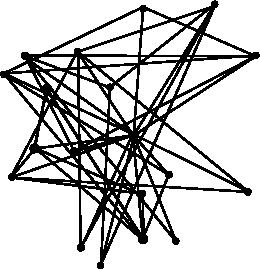
\includegraphics[width=3cm]{graph-annealing-initial.pdf}
\end{center}\pause
\begin{block}{}
\begin{center}
 Rozmístěte vrcholy grafu tak, aby graf byl co ``nejhezčí''.
\end{center}
\end{block}\pause
\begin{center}
 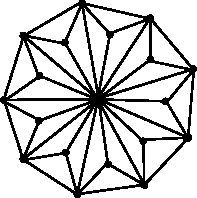
\includegraphics[width=3cm]{graph-annealing-final.pdf}
\end{center}
\end{frame}

\begin{frame}[fragile]\frametitle{Machine Learning}
\begin{center}
 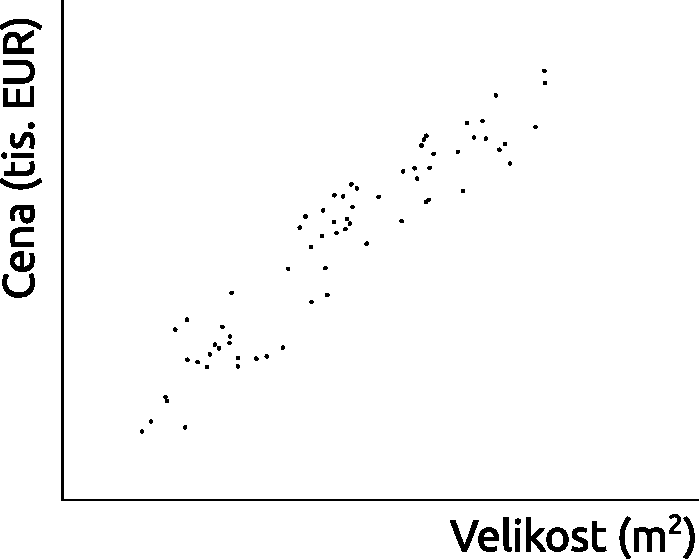
\includegraphics[width=8cm]{linear-regression-initial.pdf}
\end{center}
\end{frame}
\begin{frame}\frametitle{Machine Learning}
\begin{center}
 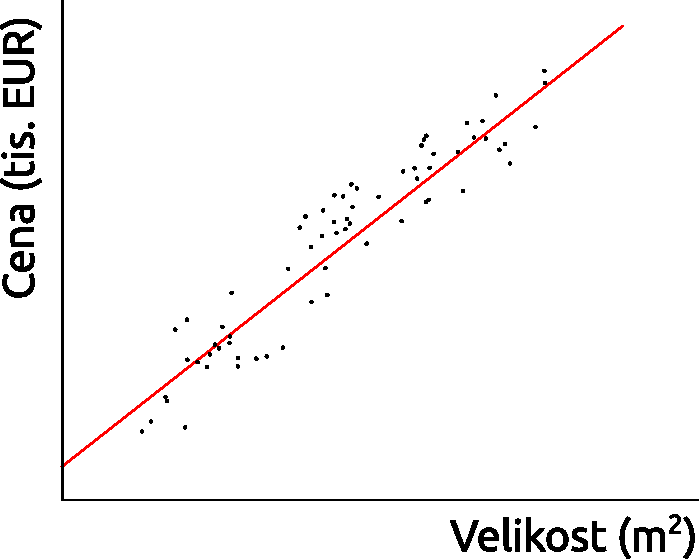
\includegraphics[width=8cm]{linear-regression-final.pdf}
\end{center}
\end{frame}

\begin{frame}\frametitle{Konstrukční problémy}
\begin{center}
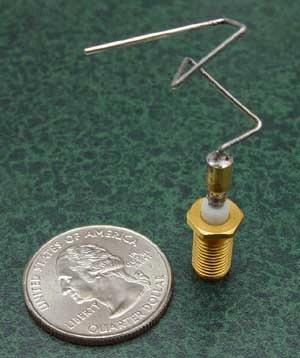
\includegraphics[width=4cm]{St_5-xband-antenna.jpg}
\end{center}
\end{frame}


\begin{frame}\frametitle{Lokální prohledávání --- algoritmy}

\begin{itemize}
 \item Horolezecká metoda (Hill-climbing)\pause
 \item Simulované žíhání (Simulated Annealing)\pause
 \item Genetické algoritmy\pause
 \item Lokální prohledávání spojitého prostoru
\end{itemize}
\end{frame}

% \begin{frame}\frametitle{Horolezecká metoda}
% \begin{block}{}
% \begin{center}
%  V každém kroku zvol nejlepšího souseda a přesuň se do něj.
% \end{center}
% \end{block}\pause
% \begin{center}
%  Problémy
% \end{center}\pause
% 
% \begin{itemize}
%  \item lokální maxima\pause
%  \item hřebeny\pause
%  \item planiny\pause
% \end{itemize}
% \end{frame}
% 
% \begin{frame}\frametitle{Hill-climbing --- varianty}
%  \begin{itemize}
%   \item první volba (FC)\pause\ --- v každém kroku zvolím prvního lepšího souseda\pause
%   \item stochastické HC\pause\  --- v každém kroku zvolím náhodně z lepších sousedů\pause\ (rozdělení může záviset na zlepšení)\pause
%   \item náhodné restartování\pause\ --- pokud neuspěji zkusím znova s jiným (náhodně zvoleným) počátečním stavem
%  \end{itemize}
% \end{frame}
% 
% 
% \begin{frame}[fragile]\frametitle{Simulované žíhání}
% Motivováno žíháním v metalurgii.\pause\ Kov (nebo sklo) se zahřeje na vysokou teplotu
% a pak se postupně chladí.\pause\ Tím je atomům umožněno získat ``lepší'' usazení v atomové mřížce.\pause
% \begin{itemize}
%  \item v každém kroku je náhodně zvolen některý soused\pause
%  \item pokud volba situaci zlepší, automaticky se tam přesuneme\pause,
%        jinak se tam přesuneme s pravděpodobností $p$\pause
%  \item pravděpodobnost $p$ závisí na \pause
%  \begin{itemize}
%    \item míře zhoršení stavu (čím větší, tím menší pravděpodobnost)\pause
%    \item iteraci (čím pozdější iterace, tím menší\pause\ --- odpovídá chladnutí)
%  \end{itemize}
% \end{itemize}\pause
%  \begin{block}{}
%  \begin{python}
%   current = pocatecni_stav()
%   while nevhodny(current):
%     soused = current.nahodny_soused()
%     delta = current.cost-soused.cost
%     if delta > 0 or random() < p(t,delta):
%       current = soused
%     t = t + 1
%  \end{python}
%  \end{block}
% 
% \end{frame}
% 
% \begin{frame}\frametitle{$k$-Lokální paprsky}
% \begin{itemize}
%  \item Místo s jedním aktuálním stavem pracujeme s $k$ stavy.\pause
%  \item V každém kroku zvolíme $k$ nových sousedů\pause
%  \item varianty stochastické, first choice, restarty
% \end{itemize}
% \end{frame}
% 
% 
% \begin{frame}\frametitle{Genetické algoritmy}
% Motivováno Darwinovou evoluční teorií.\pause\ Idea: vhodnou kombinací dobrých řešení lze získat lepší řešení.\pause\ 
% \begin{itemize}
%  \item[1.] Zvol náhodně počáteční soubor řešení, tzv. nultou generaci populace.\pause
%  \item[2.] V každém kroku \alert<7>{zvol část} aktuální generace k reprodukci.\pause
%  \item[3.] Z této části \alert<8>{vygeneruj} další generaci.\pause
%  \item[4.] Pokud je některé získané řešení dostačující skonči, jinak pokračuj krokem 2.\pause
% \end{itemize}
% \end{frame}
% 
% \begin{frame}\frametitle{Genetické algoritmy --- aplikace}
% \begin{block}{}
% \begin{center}
% Návrh radiové antény
% \end{center}
% \end{block}\pause
% 
% \begin{center}
% 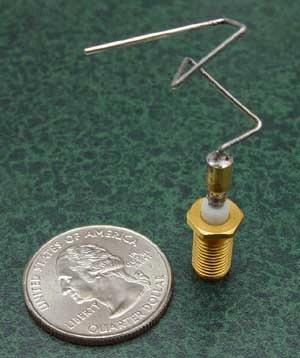
\includegraphics[width=4cm]{St_5-xband-antenna.jpg}
% \end{center}
% \end{frame}
% 
% % 
% % \begin{itemize}
% %  \item v každém kro
% % \end{itemize}
% % 
% % \begin{itemize}
% %  \item schéma --- genetický kód
% %  \item fitness
% %  \item crossover
% %  \item mutace
% % \end{itemize}
% 
% \begin{frame}\frametitle{Spojitý prostor}
% \begin{block}{}
%  Rozmístěte letiště tak, aby součet vzdáleností z okresních měst do nejbližšího letiště byl minimální.
% \end{block}\pause
%  \begin{itemize}
%   \item podobné jako hill-climbing, ale spočte se gradient a posouvá se ve směru největšího gradientu\pause
%   \item Newtonova metoda\pause
%   \item diskretizace\pause
%   \item lineární programování\pause,\ kvadratické programování\pause, konvexní optimalizace
%  \end{itemize}\pause
% \end{frame}
% 
% 
% 
% \begin{frame}[fragile]\frametitle{8-královen}
% \begin{block}{}
% \begin{center}
%  Rozmístěte na šachovnice osm dam tak, aby se žádné dvě dámy neohrožovaly.
% \end{center}
% \end{block}\pause
% \begin{center}
% Například.\pause
% 
% \setchessboard{setpieces={qa1,qb5,qc8,qd6,qe3,qf7,qg2,qh4}, showmover=false,border=false}
% \chessboard[tinyboard]
% \end{center}
% \end{frame}


\end{document}


